% Created 2017-10-24 Tue 00:38
% Intended LaTeX compiler: pdflatex
\documentclass[10pt,t]{beamer}
\usepackage[utf8]{inputenc}
\usepackage[T1]{fontenc}
\usepackage{graphicx}
\usepackage{grffile}
\usepackage{longtable}
\usepackage{wrapfig}
\usepackage{rotating}
\usepackage[normalem]{ulem}
\usepackage{amsmath}
\usepackage{textcomp}
\usepackage{amssymb}
\usepackage{capt-of}
\usepackage{hyperref}
\usetheme{default}
\author{L. Larrabee Strow, Sergio de-Souza Machado, Howard Motteler, Chris Hepplewhite, and Steven Buczkowski (UMBC)}
\date{\today}
\title{Perspectives on Building a Climate Record of AIRS+CrIS}
\date{\textit{AIRS Science Team Meeting:  \footnotesize October 24, 2017}}
\input beamer_setup
\usetheme{metropolis}
\metroset{titleformat title=allcaps}
\renewcommand{\UrlFont}{\small\tt}
\renewcommand*{\UrlFont}{\footnotesize}
\tolerance=1000
\hypersetup{
 pdfauthor={L. Larrabee Strow, Sergio de-Souza Machado, Howard Motteler, Chris Hepplewhite, and Steven Buczkowski (UMBC)},
 pdftitle={Perspectives on Building a Climate Record of AIRS+CrIS (and IASI)},
 pdfkeywords={},
 pdfsubject={},
 pdfcreator={Emacs 25.1.1 (Org mode 9.0.9)}, 
 pdflang={English}}
\begin{document}

\maketitle
\addtobeamertemplate{block begin}{
  \setlength{\parsep}{0pt}
  \setlength{\topsep}{3pt plus 2pt minus 2.5pt}
  \setlength{\itemsep}{0pt plus 0pt minus 2pt}
  \setlength{\partopsep}{2pt}
}

\section{Introduction}
\label{sec:org047a7d5}

\begin{frame}[label={sec:org648c8cc}]{Strategies for connecting AIRS and CrIS(s)}
\begin{block}{Outline}
\begin{itemize}
\item General Approach
\item Motivation and Requirements
\item Sensor Differences and Mitigation
\end{itemize}
\end{block}
\begin{block}{Themes of This Talk}
\begin{itemize}
\item Sensors stable to  <0.003K/year
\item They provide an excellent climate monitoring platform (now 15+ years).  Natural use of these data by users?
\item How will we 
\begin{enumerate}
\item Maintain stability across instruments
\item Provide users with error estimates based on sensor measurement accuracies
\end{enumerate}
\end{itemize}
\end{block}
\end{frame}


\section{General Approach}
\label{sec:orga4ad907}

\begin{frame}[label={sec:orga95dadf}]{Existing Approach}
\begin{itemize}
\item AIRS L1b ---> Retrieval ---> L3 ---> AIRS Climate?
\item CrIS L1b ---> Retrieval ---> L3 ---> CrIS Climate?
\item Combined Time series: (AIRS Climate) + (CrIS Climate)?
\end{itemize}

\begin{block}{AIRS/CrIS Retrieval Differences:}
\begin{itemize}
\item Forward models (RTA).  Hard to make them "identical".
\item Instrument Line Shapes (width, centroids), channel sensitivities, noise, channel selection
\item Spatial response (Aumann Sept. 2016 STM: 3x3 CrIS has about 8\% more variability, better Cloud-clearing?)
\item Radiometric offsets: in the 0.1-0.25K range
\end{itemize}
\end{block}
\end{frame}

\begin{frame}[label={sec:org8c8ad53}]{Proposed Strategy}
\begin{enumerate}
\item AIRS L1b ---> AIRS L1c ---> AIRS2CrIS (AIRS w/ CrIS ILS)
\item Adjust AIRS2CrIS radiometric calibration to CrIS calibration
\item Add noise to individual scenes (will vary between CrIS and AIRS2CrIS depending on wavenumber)
\end{enumerate}
\footnotesize
ILS conversion is very easy and very accurate. See Howard Mottelers talk: "AIRS deconvolution and the translation of AIRS to CrIS radiances" (3:20 PM Thursday)

\normalsize
\begin{block}{Benefits}
\begin{itemize}
\item A uniform radiance time series "cL1d" (c is for combined)
\item Provides a radiance climatology.  (Rad L3 ---> Geophysical L3).
\item \emph{Allows radiance offsets to be applied on a channel-by-channel basis for L2 retrievals}.  What is the alternative?
\item Permits use of a single forward model, removing possible paramaterization differences in fast RTAs
\item Easier system to manage, more uniformity
\end{itemize}
\end{block}
\end{frame}

\section{Motivation}
\label{sec:orgbdcb7cf}

\begin{frame}[label={sec:orgea3a5c0}]{AIRS 14-Year Global L1c BT Trends (Unc: \(\sim\) 0.003K/year)}
\begin{center}
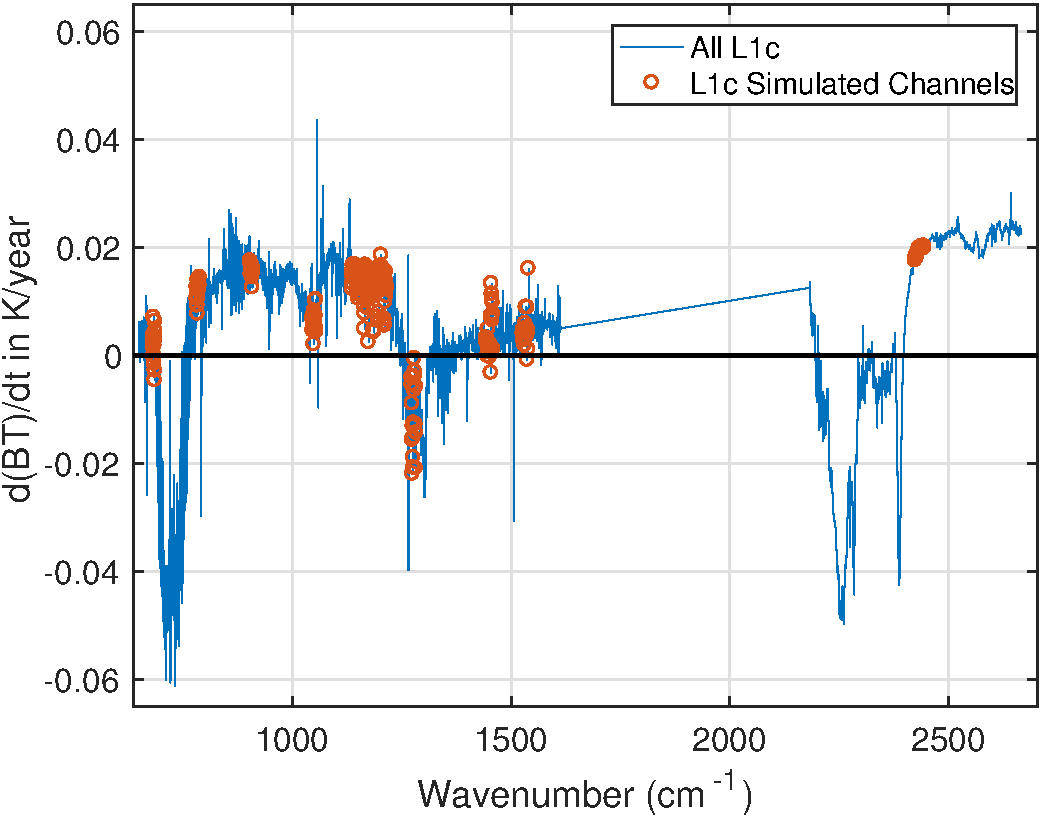
\includegraphics[width=.9\linewidth]{./Figs/Pdf/global_dbt_l1c_allchans_showfake.pdf}
\end{center}
\end{frame}
\begin{frame}[label={sec:org9dc0322}]{Effects of Greenhouse Gases on 14-Year Trends}
\vspace{-0.1in}
Long term greenhouse gas trends can be removed using in-situ data.
\begin{center}
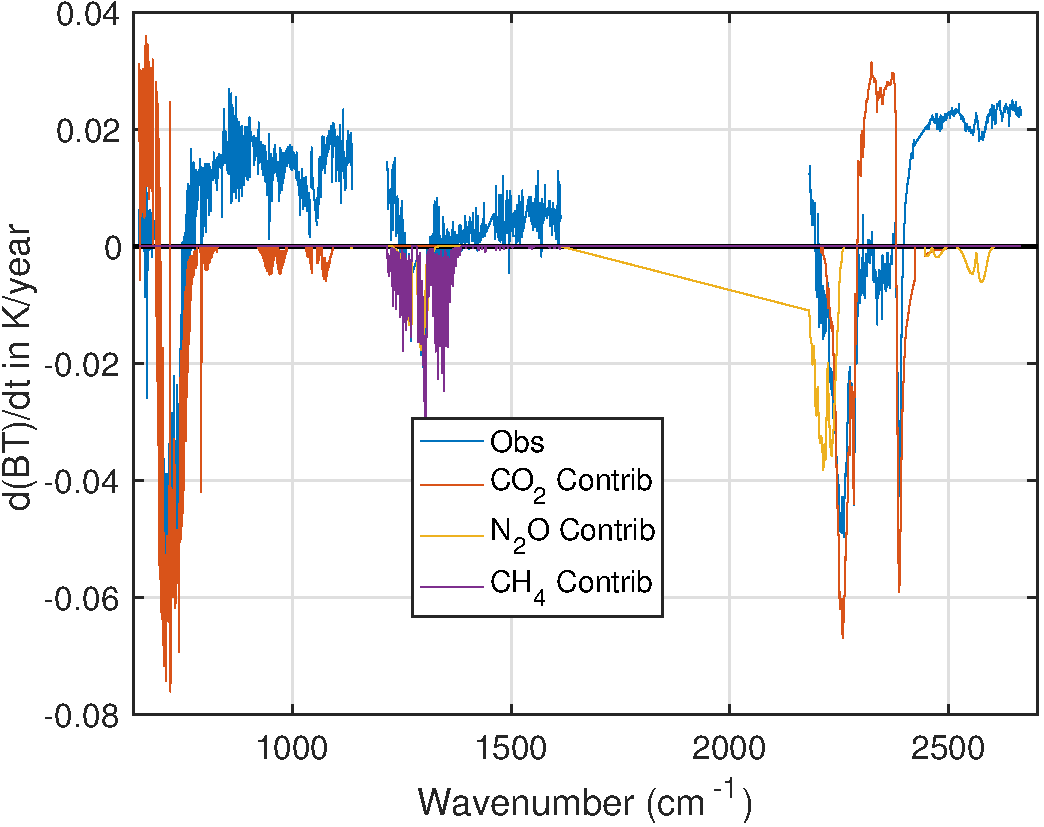
\includegraphics[width=0.8\linewidth]{./Figs/Pdf/global_dbt_l1c_withco2n2och4.pdf}
\end{center}
\end{frame}
\begin{frame}[label={sec:orgda20d96}]{14-Year Trends after Removal of Greenhouse Gases}
\vspace{-0.1in}
Surface and LW Trop. Atmospheric Trends \(\sim\) +0.01K/year
\begin{center}
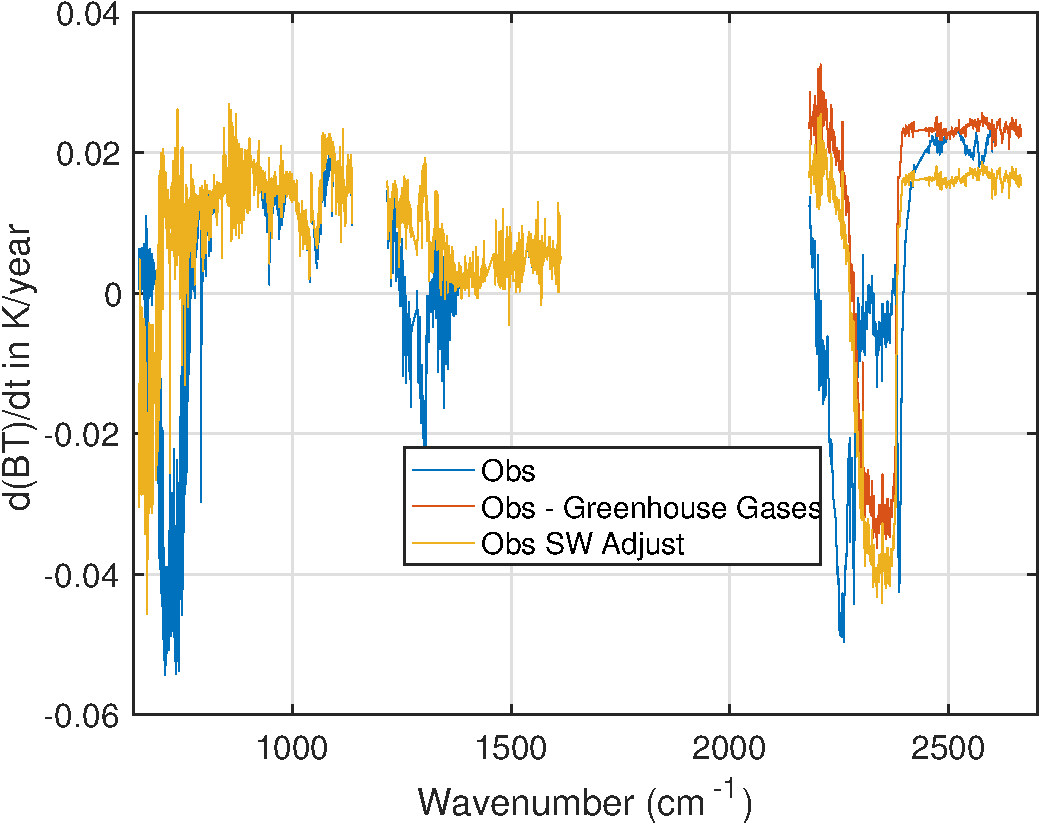
\includegraphics[width=0.8\linewidth]{./Figs/Pdf/global_dbt_l1c_minus_greenhouse_gases_swadjust.pdf}
\end{center}
\vspace{-0.1in}
\small
(SW adjusted using clear-scene SST comparisons.)
\end{frame}
\begin{frame}[label={sec:orgaa2b8d8}]{14-Year Trends Compared to ERA}
\vspace{-0.1in}
\begin{center}
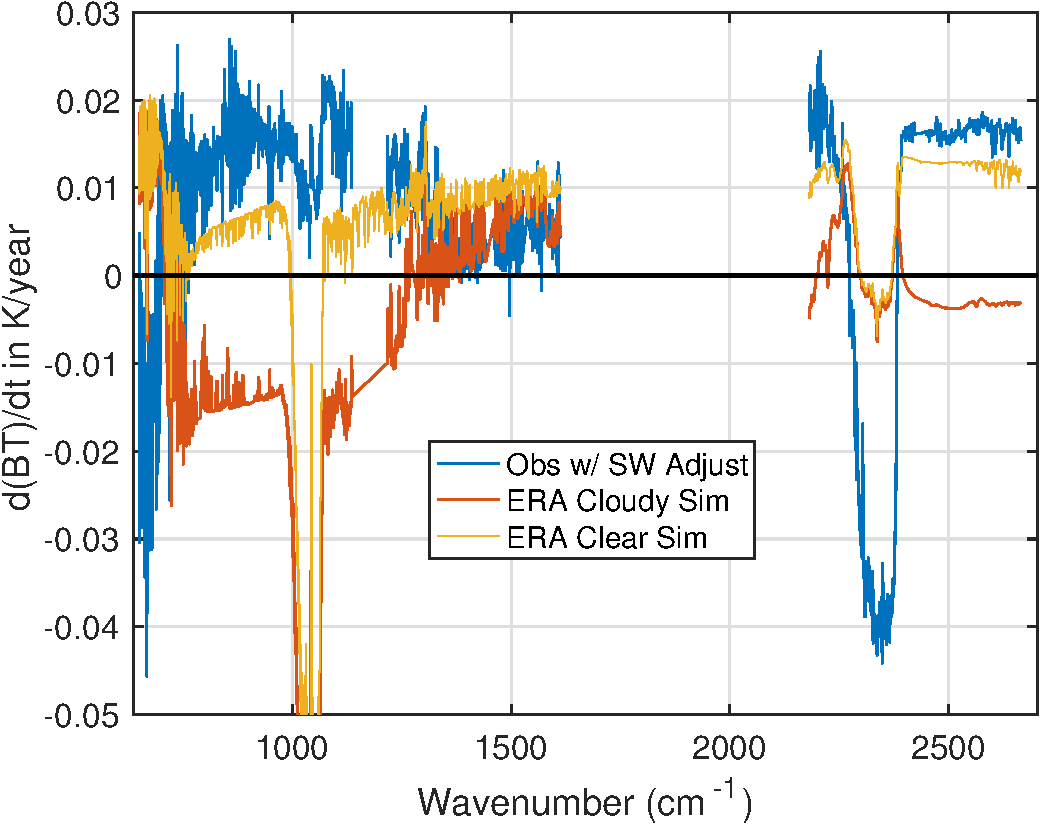
\includegraphics[width=0.8\linewidth]{./Figs/Pdf/global_dbt_l1c_with_era_cld_and_clr.pdf}
\end{center}
\vspace{-0.1in}
\small
ERA cloud trends too large.  ERA cannot tune upper strat for \cd variability??  Or, is upper strat \cd different?
\end{frame}
\begin{frame}[label={sec:org77b2448}]{Will Relative Humidity Change With Global Warming?}
\vspace{-0.1in}
\begin{center}
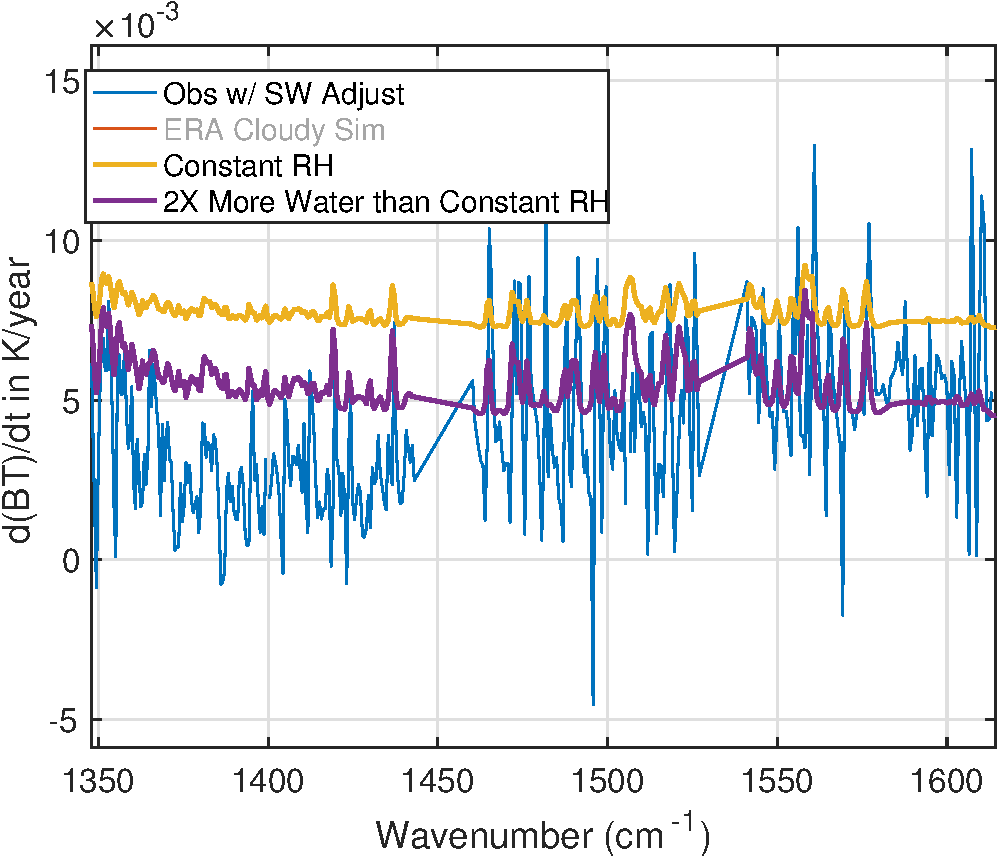
\includegraphics[width=0.8\linewidth]{./Figs/Pdf/global_dbt_l1c_minus_greenhouse_gases_swadjust_vs_era_water_RH_noera.pdf}
\end{center}
\vspace{-0.1in}
\small
This is a key climate question suitable for AIRS + CrIS
\end{frame}

\begin{frame}[label={sec:org5e53653}]{GISS vs AIRS 900 \wn B(T) Anomalies}
\vspace{-0.1in}
\begin{center}
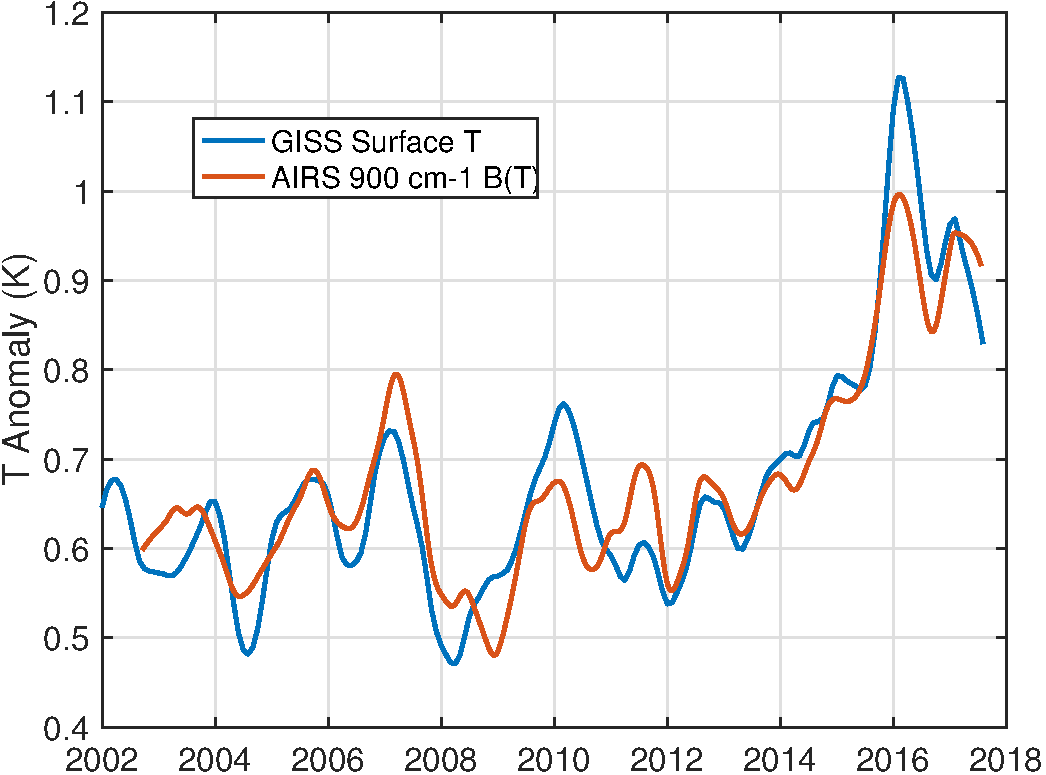
\includegraphics[width=0.8\linewidth]{./Figs/Pdf/giss_sfct_vs_airs_900cmbt.pdf}
\end{center}
\vspace{-0.05in}
\small
Changes in clouds are small (can be proven over ocean) so window channels track surface stations.  
\end{frame}

%---------------------------------------------------------------------------
\begin{frame}{Recent Warming Not Related to ENSO}

  \begin{columns}
    \begin{column}[T]{0.50\textwidth}
      \vspace{-0.2in}
      \begin{block}{\footnotesize Global 900 \wn PDF}
        \vspace{-0.1in}
        \begin{center}
          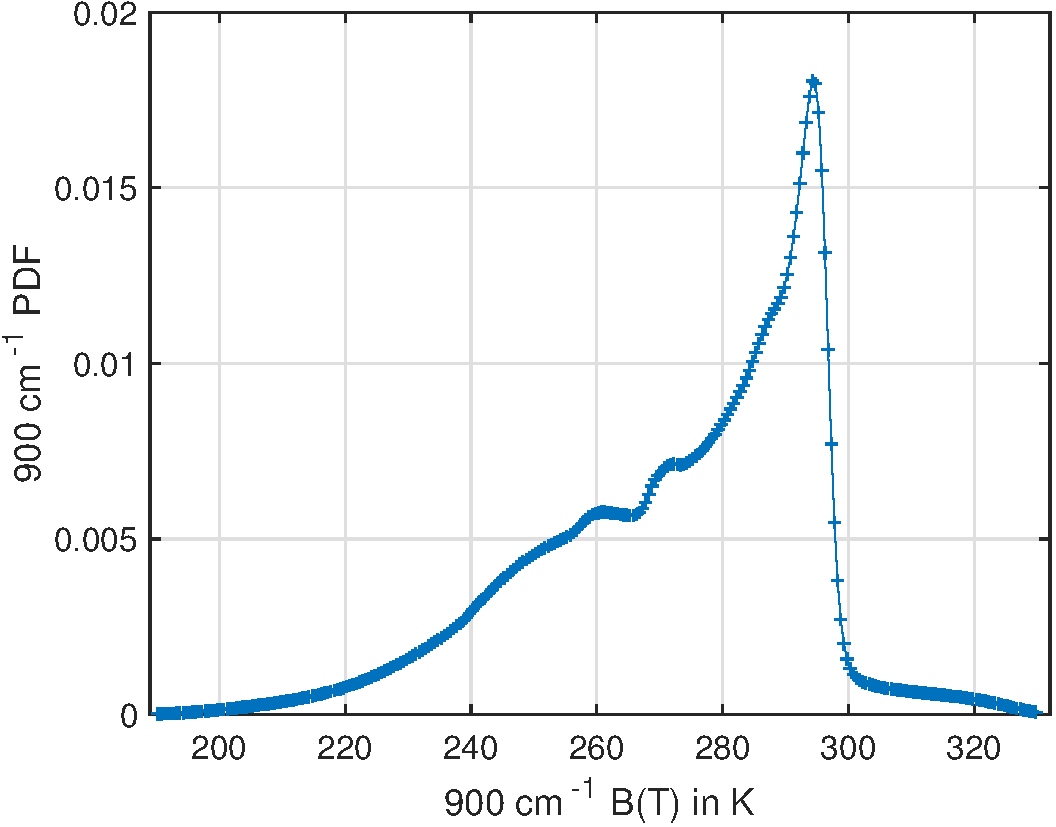
\includegraphics[width=0.80\linewidth]{./Figs_mei/Pdf/bt900_pdf_mean_in_time.pdf}
        \end{center}
      \end{block}
    \end{column}

    \begin{column}[T]{0.50\textwidth}
        \vspace{-0.2in}
      \begin{block}{\footnotesize Warmer Scene PDF Anomalies}
        \vspace{-0.1in}
        \begin{center}
          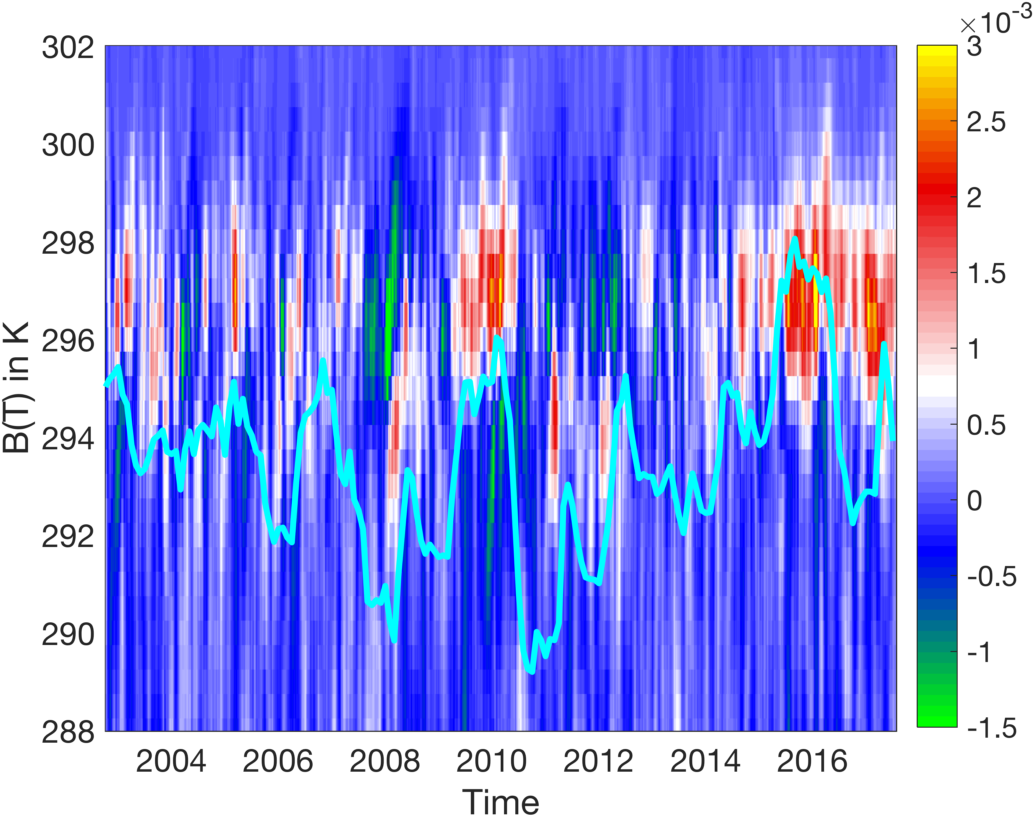
\includegraphics[width=0.80\linewidth]{./Figs_mei/Png/bt900_pdf_anom_highT_with_mei_index.png}
        \end{center}
      \end{block}
    \end{column}
  \end{columns}

  \begin{columns}
    \begin{column}{0.50\textwidth}
        \vspace{-0.2in}
      \begin{block}{\footnotesize Warming vs ENSO (MEI index)}
        \vspace{-0.1in}
        \begin{center}
%          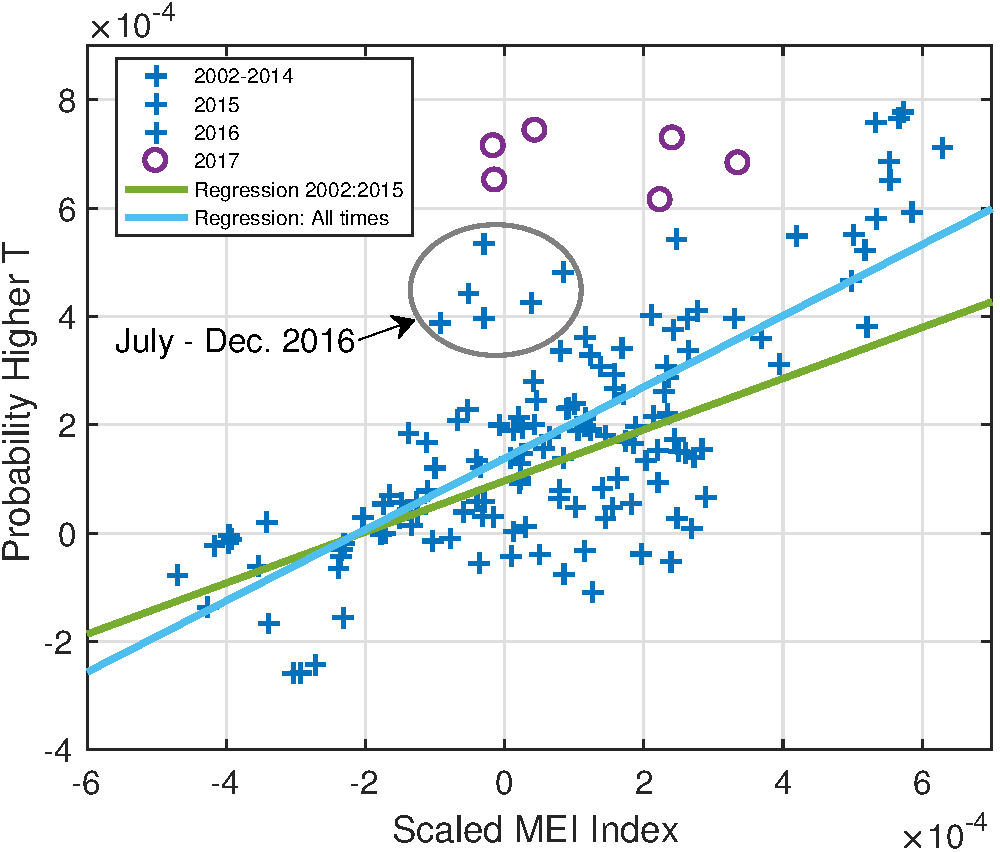
\includegraphics[width=0.80\linewidth]{./Figs_mei/Pdf/bt900_pdf_anom_highT_with_mei_index_v2_samemarker_but_2017.pdf}
          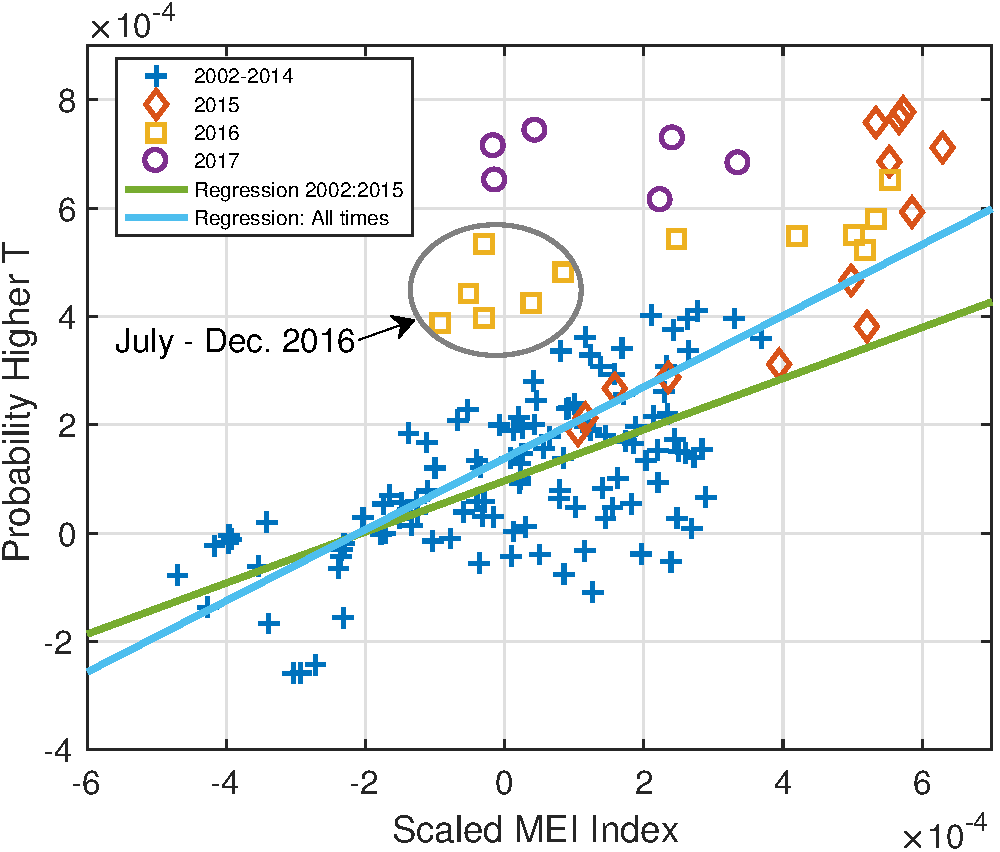
\includegraphics[width=0.85\linewidth]{./Figs_mei/Pdf/mei_vs_highT_prob_with_regr_v2.pdf}
        \end{center}
      \end{block}
    \end{column}

    \begin{column}{0.50\textwidth}
        \vspace{-0.1in}
        \begin{block}{}
        \small
        \begin{itemize}
        \item This appoach minimizes clouds (more is possible)
        \item Provides simple analysis with high certainties
        \end{itemize}
      \end{block}
    \end{column}
  \end{columns}

\end{frame}
%---------------------------------------------------------------------------



\section{Differences and Similarities Between AIRS and CrIS Radiances}
\label{sec:org4822a7d}

\begin{frame}[label={sec:org9f1eae7}]{Intercalibration Issues}
\begin{block}{Approaches}
\begin{itemize}
\item SNOs
\item Statistical comparisons of radiances
\end{itemize}
\end{block}

\begin{block}{Previous Issues}
\begin{itemize}
\item UMBC and JPL used "AIRXBCAL" like data: random nadir subsets
\item These do not provide good enough sampling for statistical intercomparisons (mostly due to time differences in scene sampling)
\item \emph{This Work:} CrIS Q/A based on imaginary radiance values too severe, we only limit min radiance (3 values for LW/MW/SW)
\item \emph{This Work:} Full all-scan sampling (every scene, yearly statistics!)
\end{itemize}
\end{block}
\end{frame}

\begin{frame}[label={sec:org62cd722}]{Full Sampling Time Differences between AIRS and SNPP-CrIS}
\begin{center}
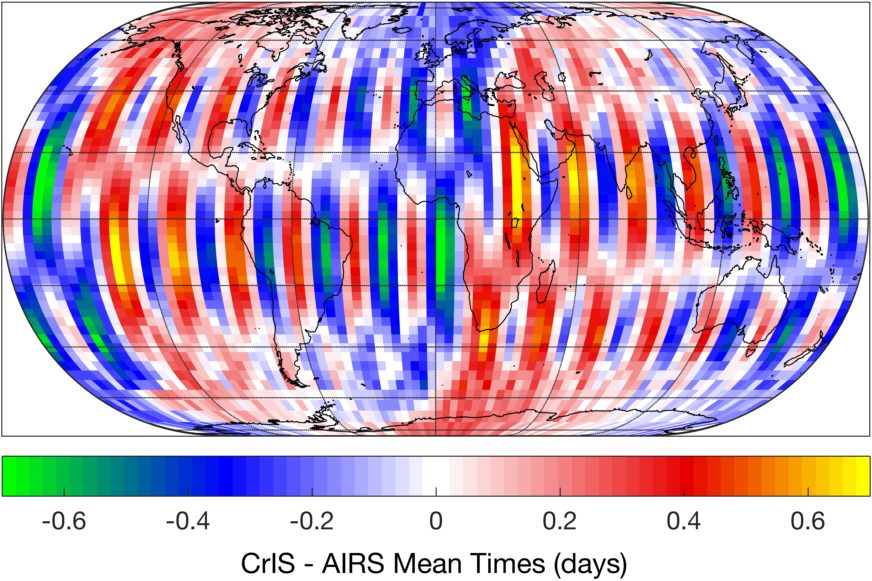
\includegraphics[width=0.8\linewidth]{./Figs/Png/airs_vs_cris_allscan_tdiff_days.png}
\end{center}

Mean global time difference is zero.  Zonal averages near zero.  Importance for retrieval products is uncertain, likely small?
\end{frame}

\begin{frame}[label={sec:orga468c42}]{AIRS vs CrIS 5-year rates: Both are Stable}
\vspace{-0.1in}
\begin{center}
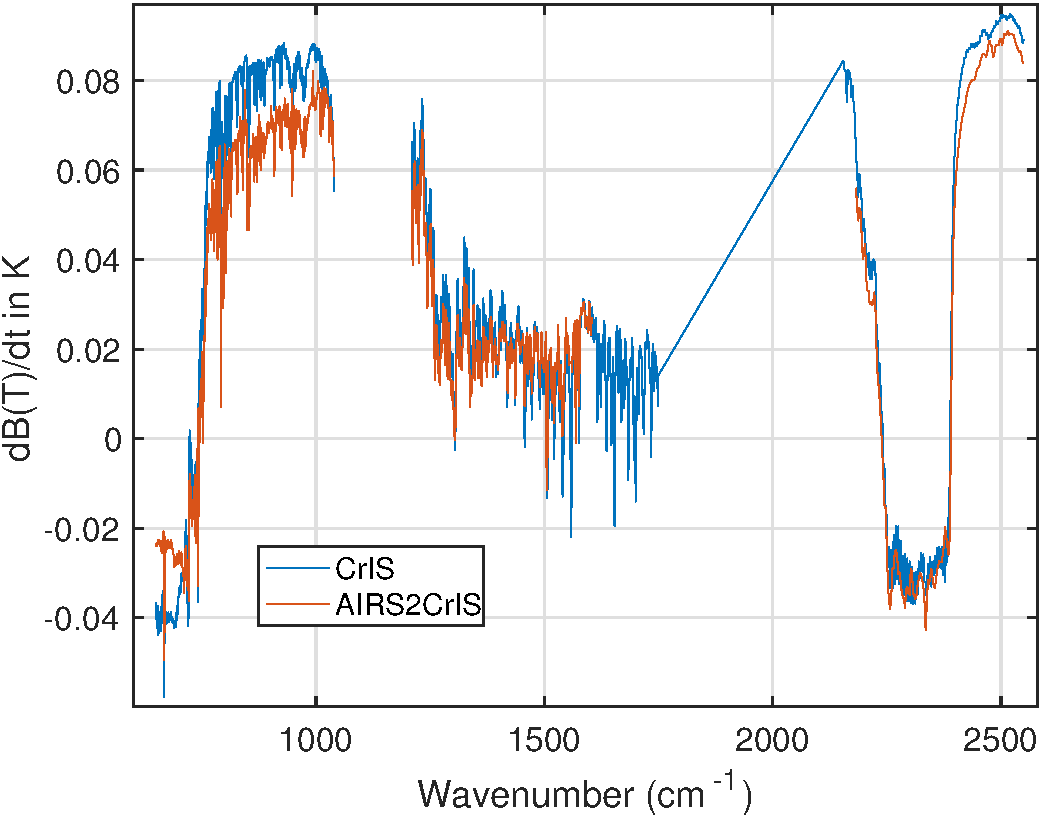
\includegraphics[width=0.8\linewidth]{./Figs/Pdf/airs_vs_cris_btrate_global.pdf}
\end{center}
Differences are far below statistical uncertainties.  Example of AIRS2CrIS.
\end{frame}

\begin{frame}[label={sec:orga10a827}]{SNO differences by AIRS Module (1-Year of SNOs)}
\vspace{-0.1in}
\begin{center}
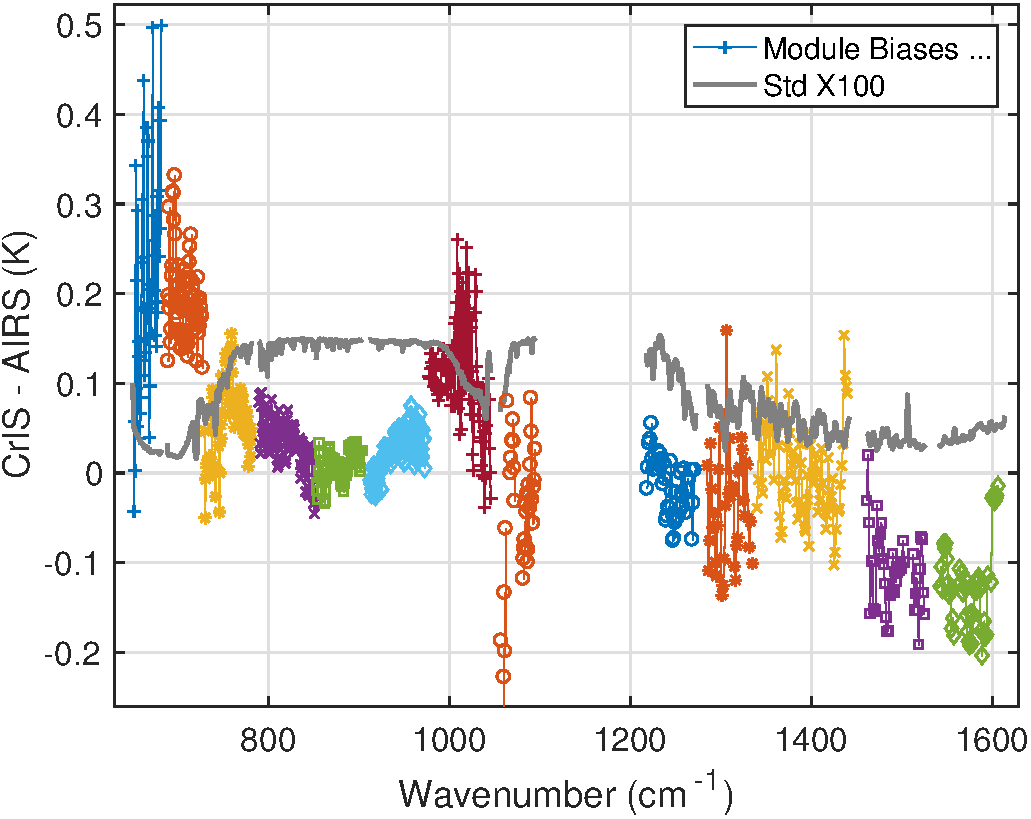
\includegraphics[width=0.8\linewidth]{./Figs/Pdf/lls_cris_minus_airs.pdf}
\end{center}
\vspace{-0.05in}
\small
AIRS2CrIS shown. Statistical errors very small.  Small scale variability likely AIRS ILS uncertainties!
\end{frame}

\begin{frame}[label={sec:orgdf19c22}]{Use SNOs to Improve AIRS Longwave ILS?}
\vspace{-0.15in}
\begin{center}
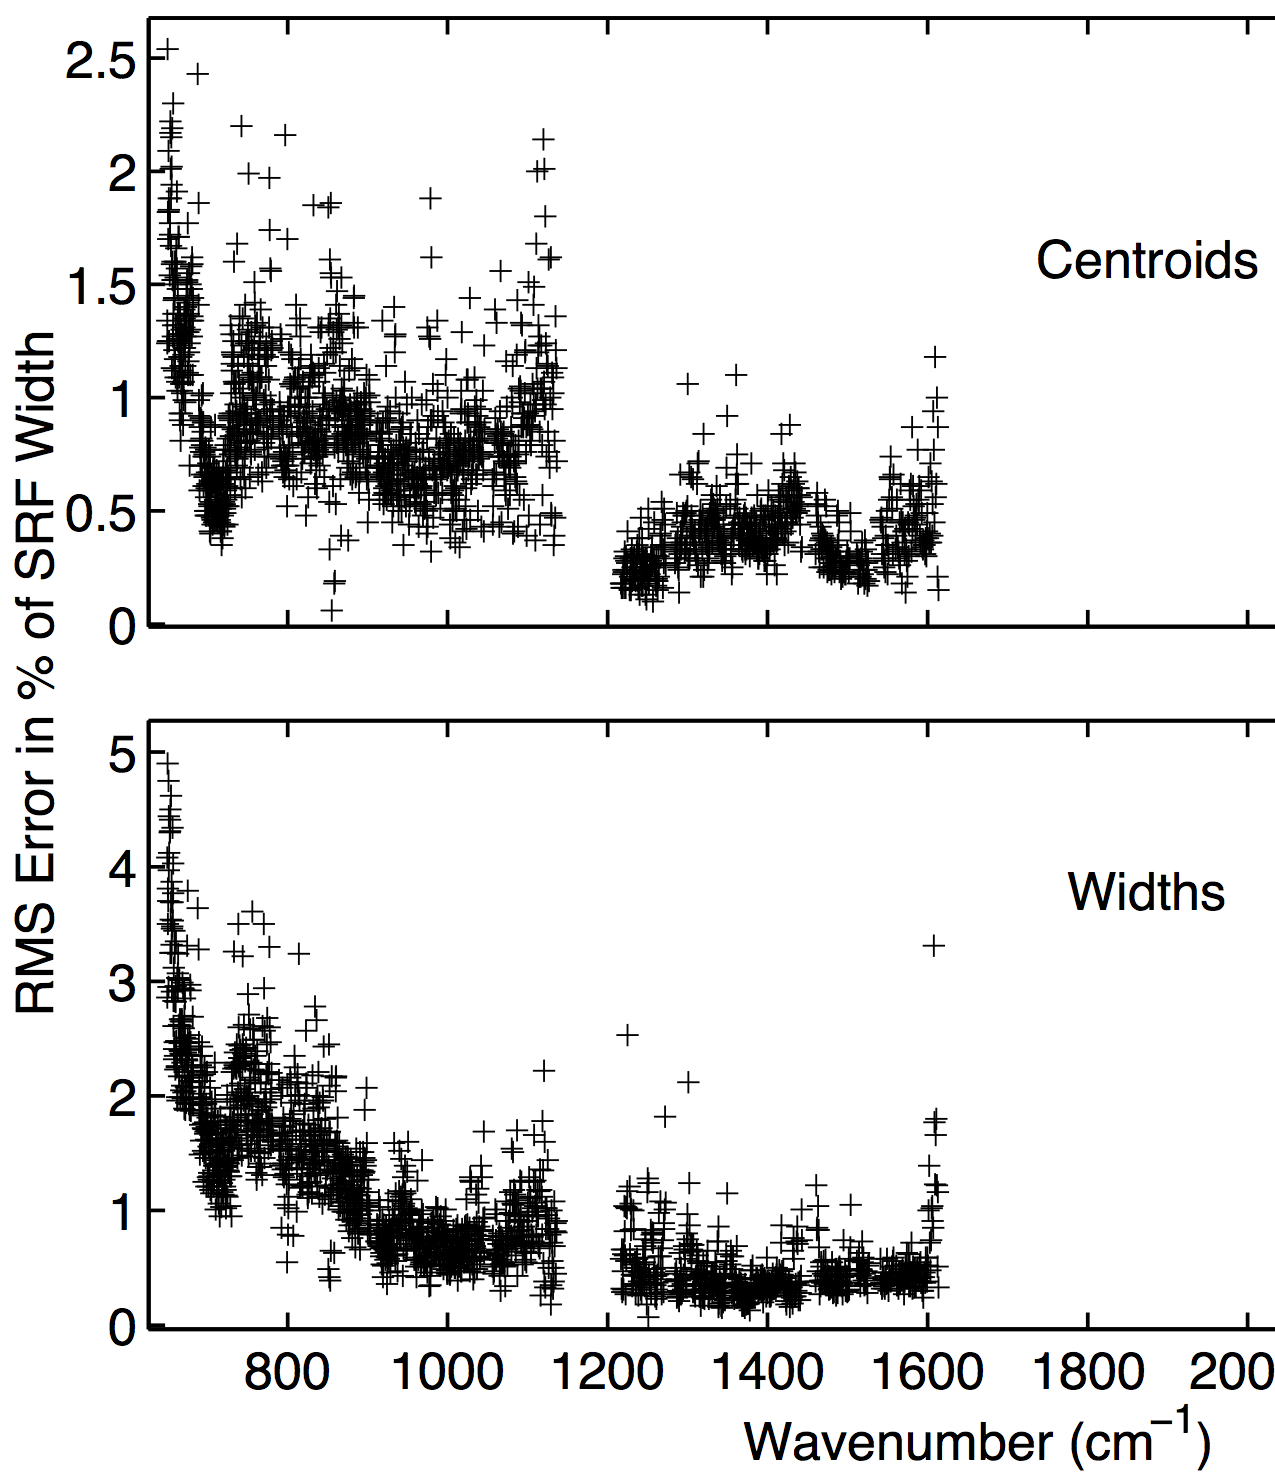
\includegraphics[width=0.6\linewidth]{./center-width-rms-err.png}
\end{center}
\end{frame}

\begin{frame}[label={sec:org69bb52a}]{Longwave Count Histograms (700 Million per Year)}
\begin{center}
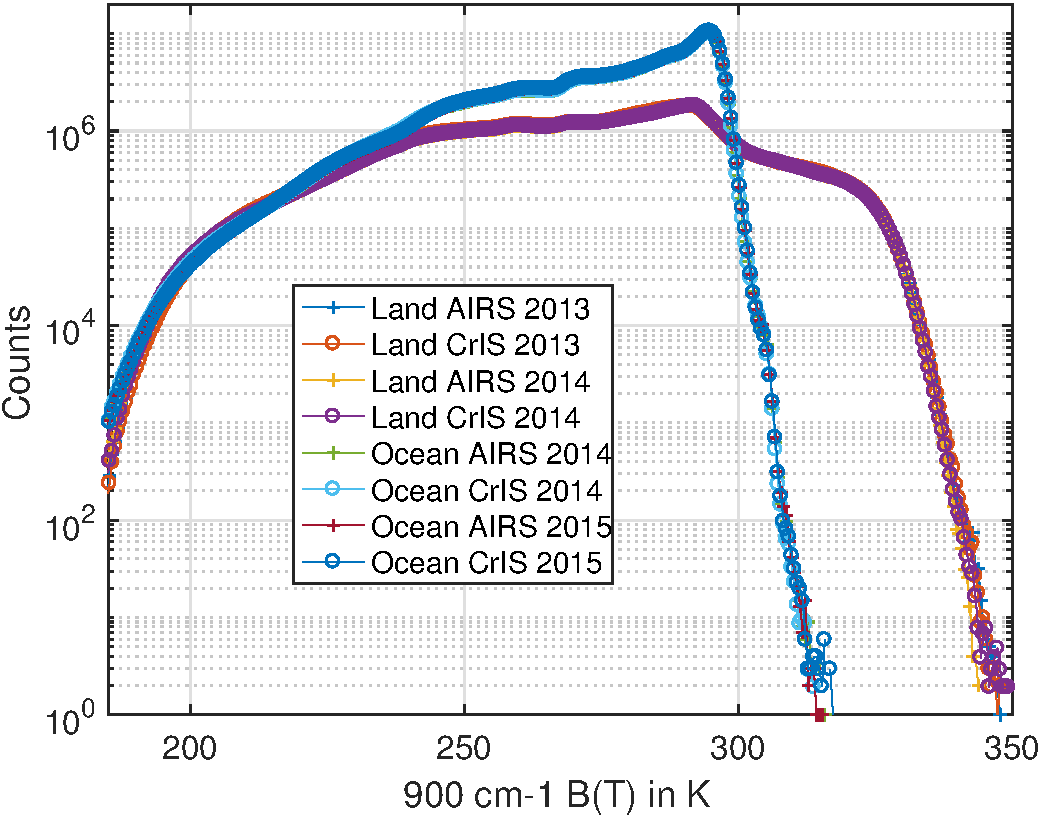
\includegraphics[width=0.7\linewidth]{./Figs/Pdf/land_and_ocean_allT.pdf}
\end{center}
\vspace{-0.15in}
\small
Not land counts only agree with change in CrIS Q/C
\end{frame}

\begin{frame}[label={sec:orgaa004ae}]{Longwave Ocean Count Differences (due to spatial diffs?)}
\begin{center}
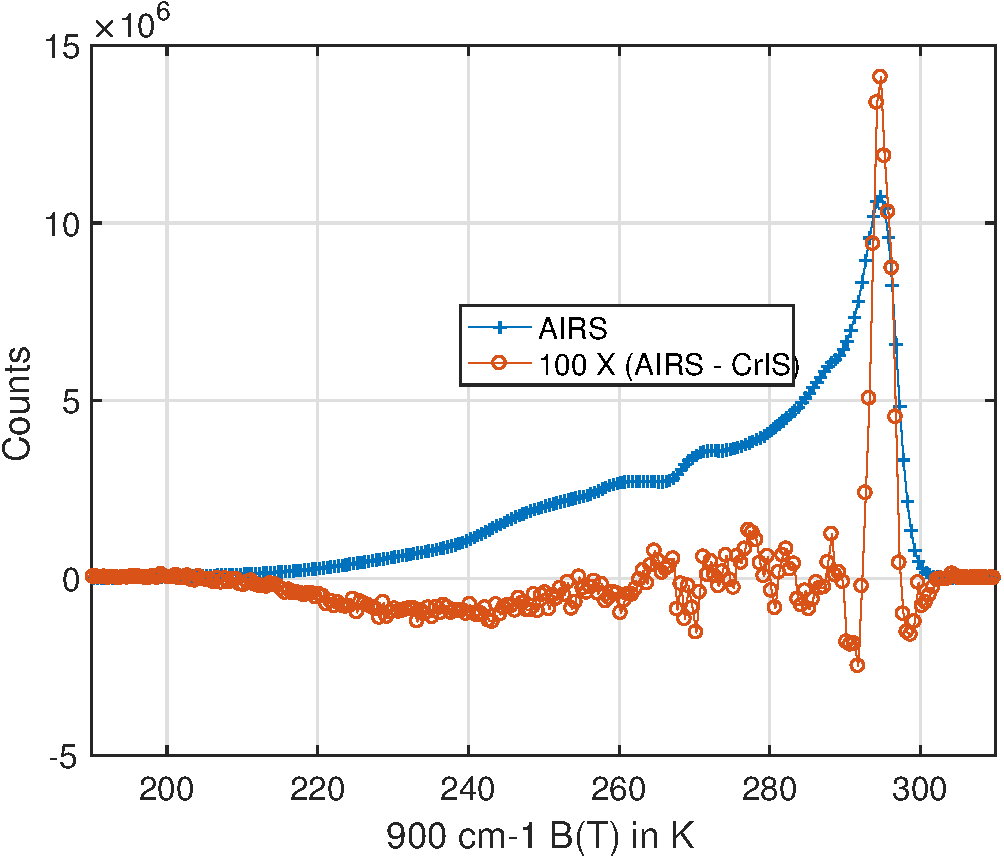
\includegraphics[width=0.7\linewidth]{./Figs/Pdf/ocean_linear_pdf_and_diff.pdf}
\end{center}
\vspace{-0.15in}
\small
AIRS FOV is slightly smeared relative to the CrIS FOV.
\end{frame}

\begin{frame}[label={sec:orgf21917b}]{Longwave Counts Vary More with Year than \\Between Instruments}
\begin{center}
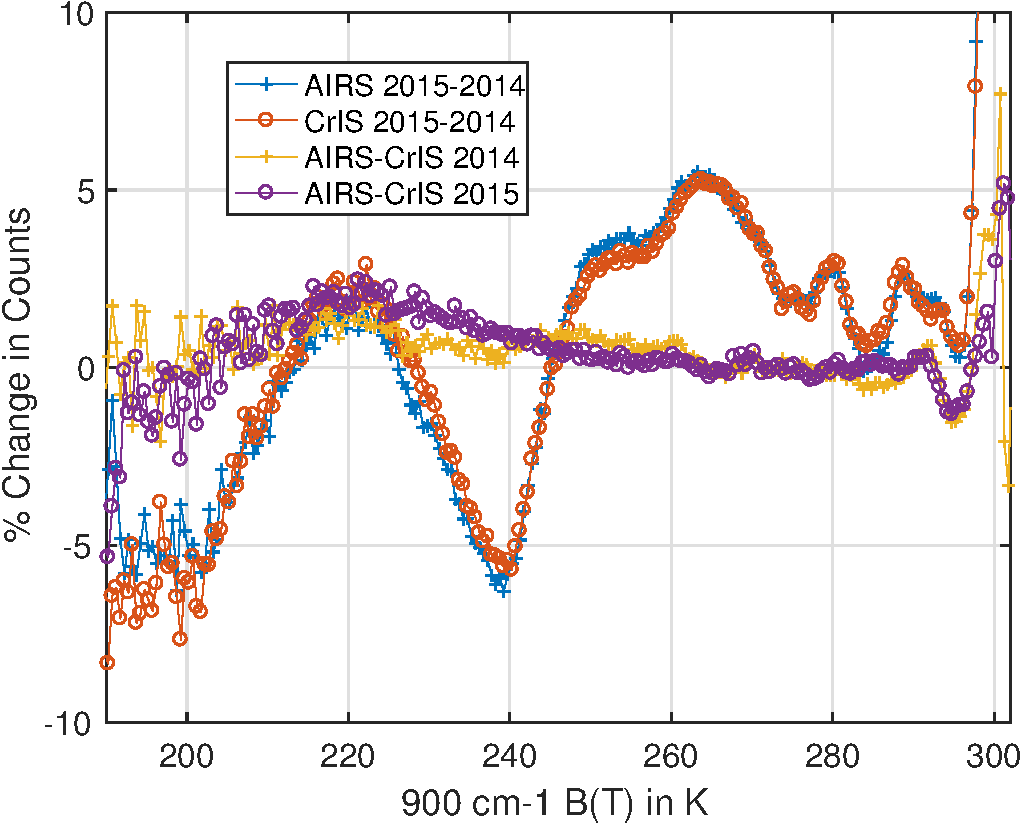
\includegraphics[width=0.8\linewidth]{./Figs/Pdf/ocean_percent_count_changes.pdf}
\end{center}
\end{frame}

\begin{frame}[label={sec:org86b7c90}]{Hot Scene Shortwave Histograms (solar reflection off clouds)}
\begin{center}
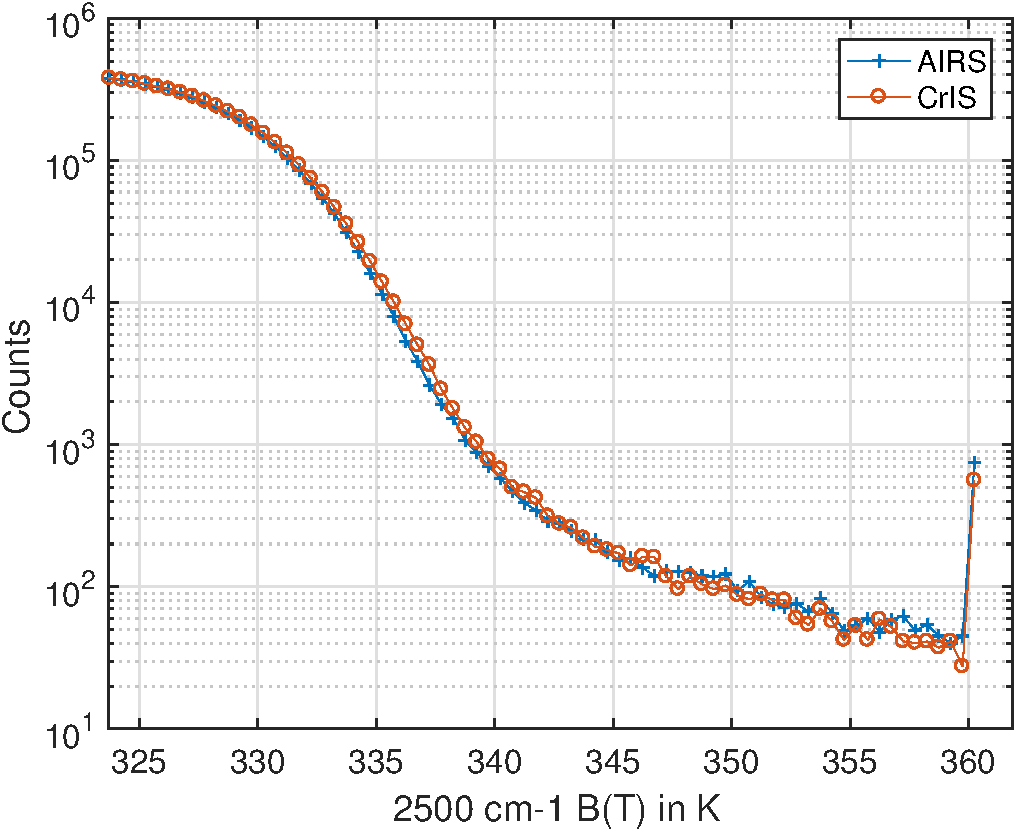
\includegraphics[width=0.7\linewidth]{./Figs/Pdf/global_sw_counts_bt325plus.pdf}
\end{center}
\vspace{-0.05in}
\small
CrIS stopped far below max before change in CrIS Q/C.  This is a remarkable
result!
\end{frame}

\begin{frame}[label={sec:org1dc5792}]{Do AIRS2CrIS and CrIS Have Simiar Count Spectra?}
\small Random Sampled AIRS L1c and AIRS2CrIS for 1 Day
\begin{center}
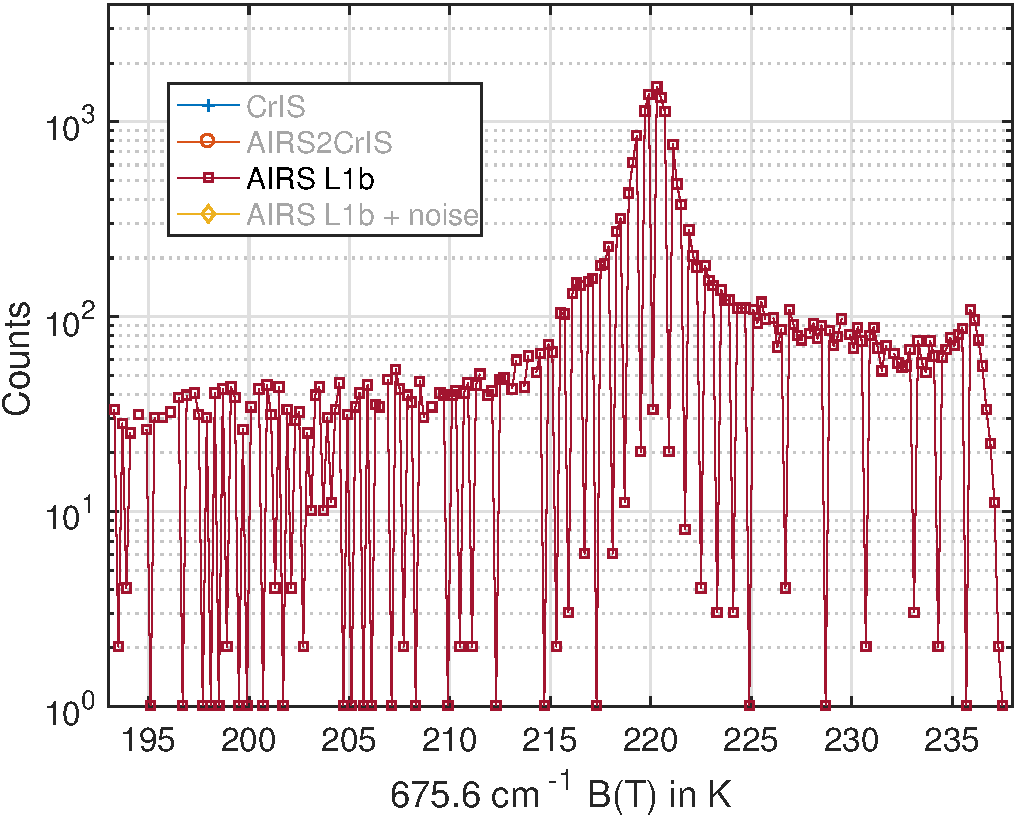
\includegraphics[width=0.7\linewidth]{./Figs/Pdf/jun4_2015_airs_675wn_global_counts.pdf}
\end{center}
\end{frame}
\begin{frame}[label={sec:org2841d2a}]{Add Noise to AIRS (L1b/c radiances are rounded)}
\begin{center}
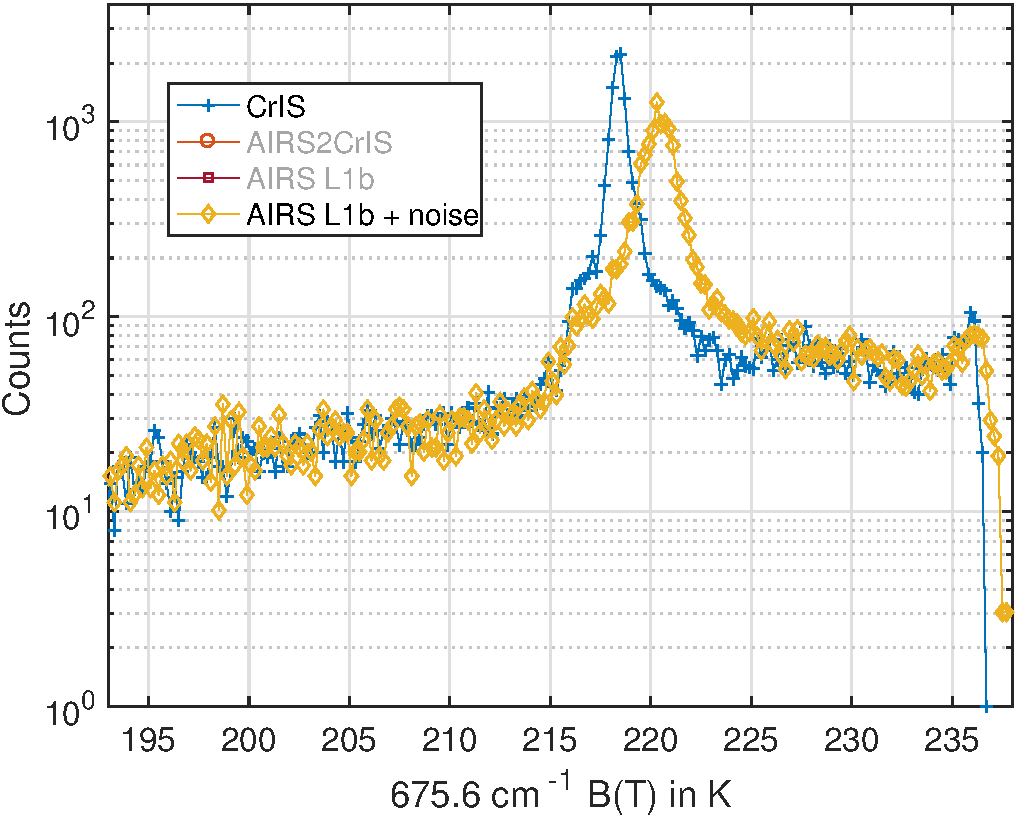
\includegraphics[width=0.8\linewidth]{./Figs/Pdf/jun4_2015_airs_675wn_global_counts_w_airsnoise_and_cris.pdf}
\end{center}
\end{frame}
\begin{frame}[label={sec:orgc445909}]{Now Compare CrIS counts to AIRS2CrIS}
\begin{center}
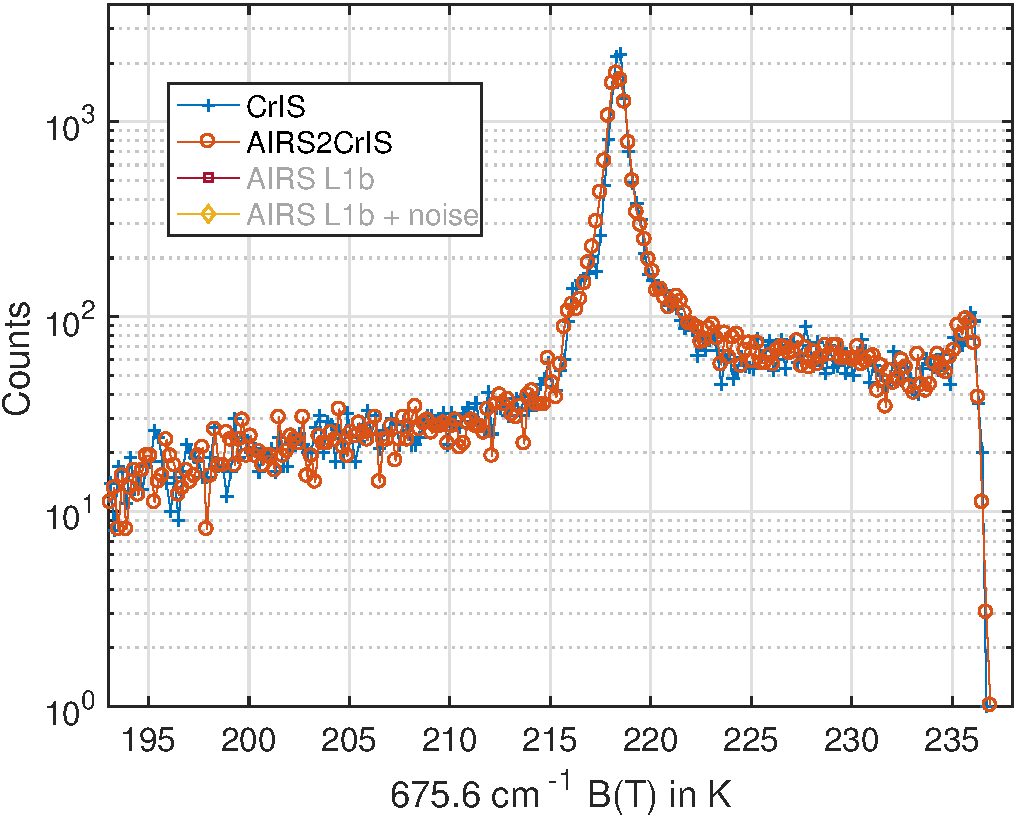
\includegraphics[width=0.7\linewidth]{./Figs/Pdf/jun4_2015_airs_675wn_global_counts_w_airsnoise_and_cris_a2c_no_airs.pdf}
\end{center}
\vspace{-0.05in}
\small
Very similar, note how sharp drop in AIRS hot wing now agrees with CrIS.
\end{frame}

\begin{frame}[label={sec:orgb04bdc0}]{Conclusions}
\vspace{-0.10in}
\small
\begin{block}{UMBC: Next Steps}
\begin{itemize}
\item Test climate level trends and anomalies between AIRS and AIRS2CrIS
\begin{itemize}
\item Create 10-year AIRS T/Q trends based on radiance trends
\item Create 5-year AIRS + 5-Year CrIS radiance product and then compare T/Q trends from this product to the AIRS-only product
\end{itemize}
\item Spectral calibration of AIRS L1c so variable \(\nu\) RTA is not needed
\end{itemize}
\end{block}

\begin{block}{Sounder SIPS and Science Team}
\begin{itemize}
\item Consider using AIRS2CrIS?
\item Should simplify retrieval system, not unimportant in time of diminishing funds
\item Will allow us to produce a combined, homogenous radiance record for future research
\item AIRS2CrIS is the only way I know to easily remove radiometric calibration differences between AIRS and CrIS.  We should not just "eat" this difference and plow ahead.
\end{itemize}
\end{block}
\end{frame}
\end{document}
%%% Local Variables:
%%% mode: latex
%%% TeX-master: t
%%% End:
